\section{The specification determines the variation used to estimate the coefficient}
\subsection{Estimate, translate, compare}

\begin{frame}{Pooled OLS summarizes the plotted association}
  \centering
  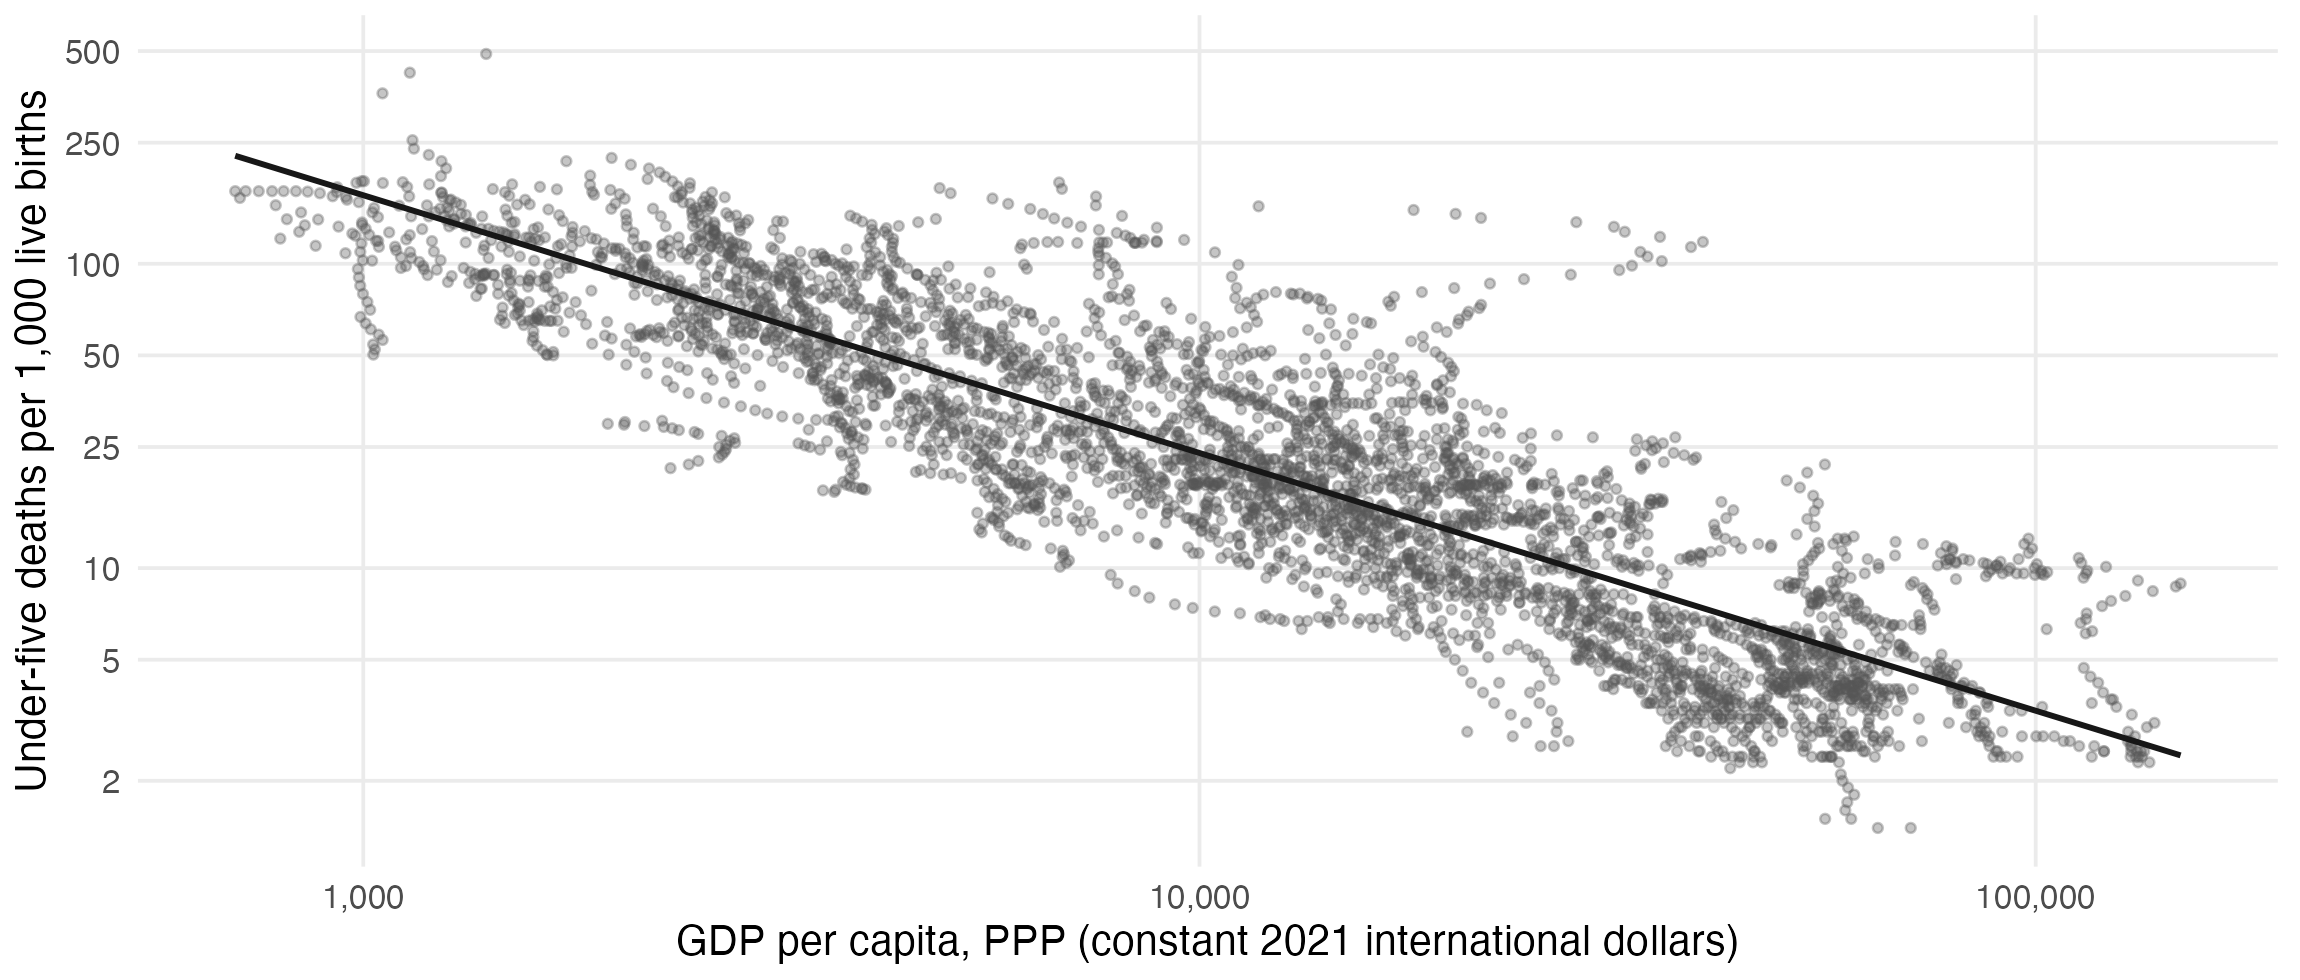
\includegraphics[width=0.92\textwidth,keepaspectratio]{figures/03-pooled-fit.png}
  \fnote{Source: World Bank, World Development Indicators. The fitted line uses
  all observed economy--years and both variables in logarithms.}
\end{frame}

\begin{frame}[fragile]{Fit the pooled association in RStudio}
  Predict the sign of \texttt{log\_income}. Then run the model and record the
  coefficient and sample size.

\begin{lstlisting}[language=R]
fit_pooled <- lm(
  log_mortality ~ log_income,
  data = health_panel
)

summary(fit_pooled)
\end{lstlisting}

  The model uses the same 4,296 observations shown in the plot.
\end{frame}

\begin{frame}{Choose the correct interpretation}
  \begin{columns}[T,onlytextwidth]
    \column{0.76\textwidth}
      \textbf{Slido multiple choice}

      Which sentence accurately reports the pooled estimate?
      \begin{enumerate}
        \item Across observed economy--years in 2000--2022, 10\% higher GDP per
          capita is associated with about 7.8\% lower under-five mortality on average.
        \item Across observed economy--years, 10\% higher GDP per capita is
          associated with 7.8 fewer deaths per 1,000 live births.
        \item Within the same economy over time, 10\% higher GDP per capita is
          associated with 7.8\% lower mortality.
        \item A 10\% increase in GDP per capita reduces under-five mortality by 7.8\%.
      \end{enumerate}
    \column{0.20\textwidth}
      \onslide<1->{%
  \begin{center}
    \href{https://sli.do/2209653}{%
      
\includegraphics[width=2.45cm]{figures/slido-lesson-3-qr.png}%
    }

    \vspace{0.25em}
    {\scriptsize\href{https://sli.do/2209653}{\textbf{Join at sli.do}}\par}
    {\small\texttt{\#2209653}\par}
  \end{center}%
}

  \end{columns}
\end{frame}

\begin{frame}{Translate the log--log coefficient}
  The pooled coefficient on \texttt{log\_income} is approximately
  \(-0.847\).

  \vspace{0.5em}
  For a 10\% income difference:
  \[
    100\left[\exp\{\widehat\beta\log(1.10)\}-1\right]
    \approx -7.8\%.
  \]

  Across observed economy--years during 2000--2022, 10\% higher GDP per capita
  is associated with roughly 7.8\% lower under-five mortality on average.

\end{frame}

\begin{frame}{Predict the fixed-effects comparison}
  \begin{columns}[T,onlytextwidth]
    \column{0.76\textwidth}
      \textbf{Slido multiple choice}

      After economy and year fixed effects are added, which variation identifies
      the income coefficient, and how do you expect its magnitude to compare
      with pooled OLS?
      \begin{enumerate}
        \item Within-economy changes after common year movements; smaller
          magnitude than pooled OLS.
        \item Cross-economy comparisons within a calendar year; approximately
          the same magnitude as pooled OLS.
        \item Changes in the global annual mean; larger magnitude than pooled OLS.
        \item Economies observed in 2022; a coefficient of zero.
      \end{enumerate}
    \column{0.20\textwidth}
      \onslide<1->{%
  \begin{center}
    \href{https://sli.do/2209653}{%
      
\includegraphics[width=2.45cm]{figures/slido-lesson-3-qr.png}%
    }

    \vspace{0.25em}
    {\scriptsize\href{https://sli.do/2209653}{\textbf{Join at sli.do}}\par}
    {\small\texttt{\#2209653}\par}
  \end{center}%
}

  \end{columns}
\end{frame}

\begin{frame}{Three specifications use different sources of variation}
  \begin{enumerate}
    \item \textbf{Pooled OLS: comparisons across all economy--years.}\par
      Persistent economy differences and year movements contribute.
    \item \textbf{Year fixed effects: economies compared within a calendar year.}\par
      Common year movements are absorbed. Persistent economy differences remain.
    \item \textbf{Economy and year fixed effects: changes within economies.}\par
      Economy levels and year movements are absorbed. Other covariates may
      still change.
  \end{enumerate}

  \vfill
  Each specification is descriptive. The variation used to estimate the income
  coefficient changes.
\end{frame}

\begin{frame}[fragile]{Change the specification in RStudio}
\begin{lstlisting}[language=R]
fit_year_fe <- lm(
  log_mortality ~ log_income + factor(year),
  data = health_panel
)

fit_economy_year_fe <- lm(
  log_mortality ~ log_income +
    factor(iso3c) + factor(year),
  data = health_panel
)
\end{lstlisting}

\end{frame}

\begin{frame}{The within-economy estimate is smaller}
  \centering
  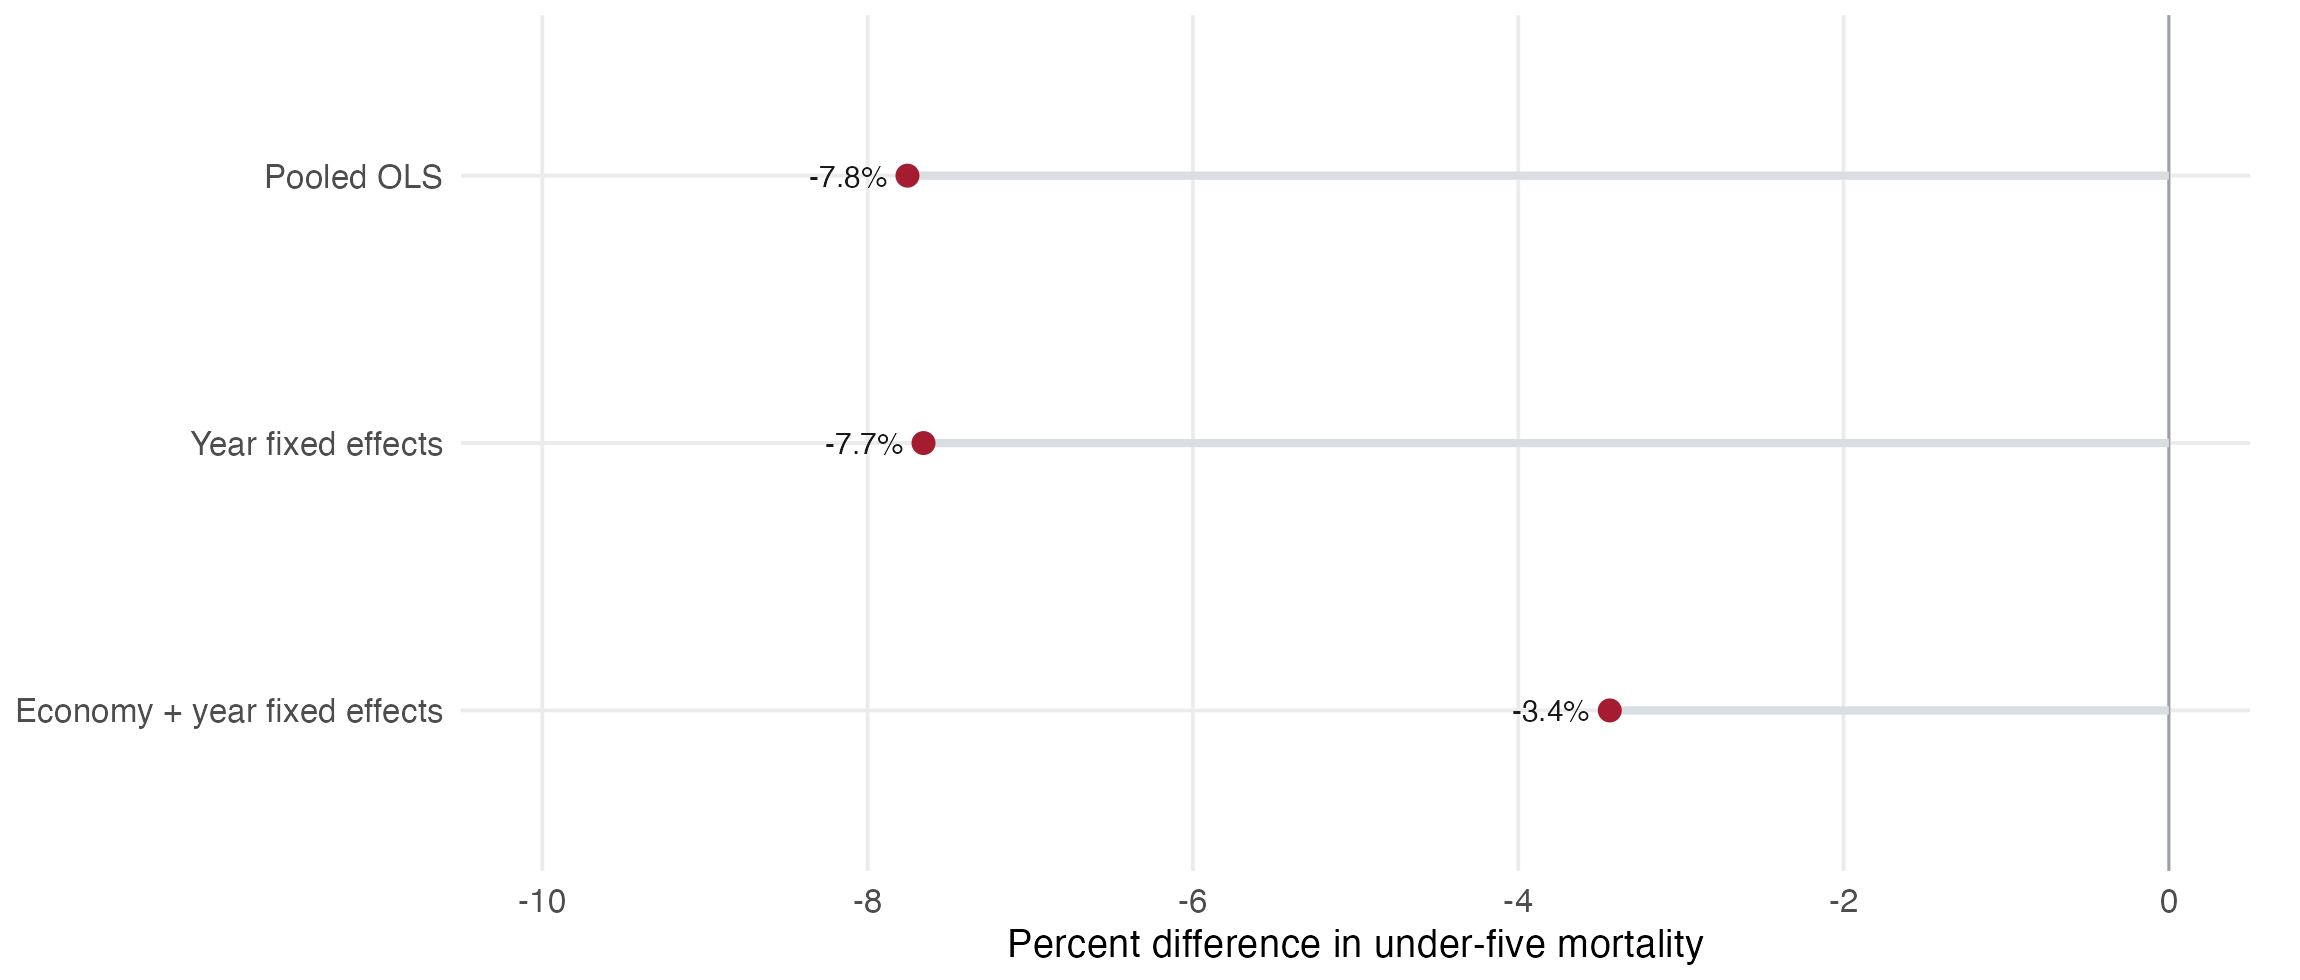
\includegraphics[width=0.94\textwidth,keepaspectratio]{figures/04-model-comparison.png}
  \fnote{Source: authors' calculations using World Bank World Development
  Indicators. Each estimate reports the mortality difference associated with
  10\% higher GDP per capita.}
\end{frame}

\begin{frame}{Interpret the three estimates}
  \begin{itemize}
    \item \textbf{Pooled OLS:} about \(-7.8\%\) across all economy--years.
    \item \textbf{Year fixed effects:} about \(-7.7\%\) across economies observed
      in the same calendar year.
    \item \textbf{Economy and year fixed effects:} about \(-3.4\%\) from changes
      within economies after common year movements.
  \end{itemize}

  \vspace{0.7em}
  Year fixed effects barely change the pooled estimate. Adding economy fixed
  effects reduces the coefficient substantially. Persistent cross-economy
  differences account for most of the change across specifications.

  \vfill
  The figure reports point estimates. Inference requires standard errors that
  allow for dependence within economies.
\end{frame}

\begin{frame}{Checkpoint 2: draft a three-sentence briefing}
  With a partner, write exactly three sentences:
  \begin{enumerate}
    \item Report the pooled estimate in percentage units.
    \item Report how the economy and year fixed-effects estimate differs and
      state which comparisons changed.
    \item State the principal research-design limitation.
  \end{enumerate}

  \vfill
  \centering
  \textbf{2 minutes discuss}\qquad$\longrightarrow$\qquad
  \textbf{2 minutes share}
\end{frame}

\begin{frame}{Checkpoint 2: model briefing}
  Across 4,296 observed economy--years during 2000--2022, 10\% higher GDP per
  capita is associated with about 7.8\% lower under-five mortality on average.

  \vspace{0.6em}
  With economy and year fixed effects, the corresponding association is about
  3.4\%; this coefficient uses changes within economies after accounting for
  common year movements.

  \vspace{0.6em}
  Other time-varying determinants remain, so these estimates do not identify
  the effect of an income intervention.

\end{frame}

\begin{frame}{Equatorial Guinea departs sharply from the pooled prediction}
  \centering
  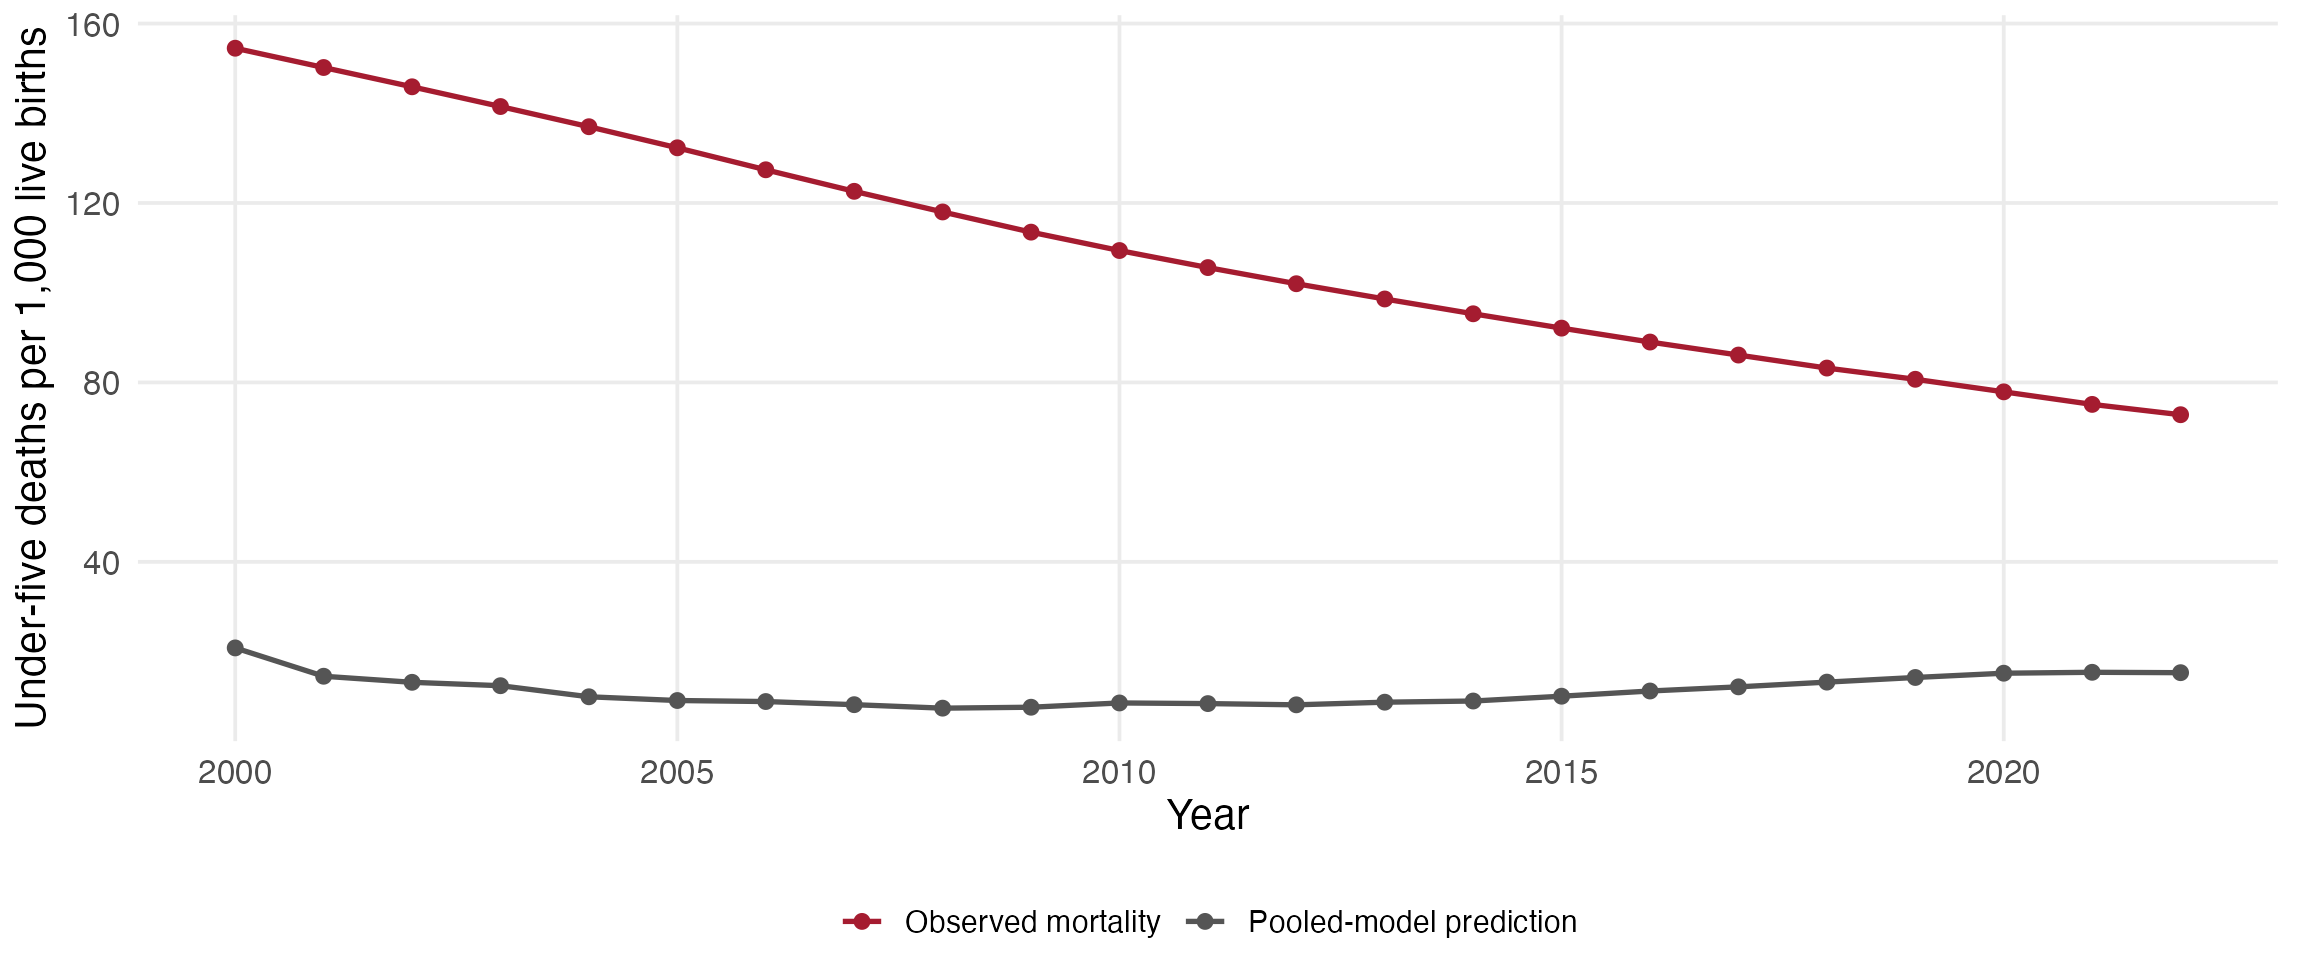
\includegraphics[width=0.94\textwidth,keepaspectratio]{figures/05-case-trajectory.png}
  \fnote{Source: World Bank, World Development Indicators, and authors'
  calculations. The gray series applies the pooled log--log specification to
  Equatorial Guinea's reported GDP per capita in each year.}
\end{frame}

\begin{frame}{The country case raises additional policy questions}
  In 2008, Equatorial Guinea's reported GDP per capita was approximately
  \$39,995 in constant PPP terms. Under-five mortality was 118 deaths per 1,000
  live births; the pooled model predicted approximately 7.4.

  \vspace{0.6em}
  Before explaining the discrepancy, investigate:
  \begin{enumerate}
    \item the definitions, units, and construction of both indicators;
    \item how national income was distributed across households;
    \item access to primary care, sanitation, nutrition, and maternal services;
    \item the timing between changes in income and changes in health systems;
    \item whether the pooled functional form represents this country's trajectory.
  \end{enumerate}

  \vfill
  The figure establishes a large difference between the observed outcome and
  the pooled prediction. Explaining that difference requires additional data.
\end{frame}

\begin{frame}{Does one observation drive the pooled estimate?}
  Remove Equatorial Guinea--2008, refit the same pooled specification, and
  compare the reported 10\% income difference.

  \vspace{0.6em}
  \renewcommand{\arraystretch}{1.4}
  \begin{tabularx}{\textwidth}{@{}>{\RaggedRight\arraybackslash}Xrr@{}}
    \toprule
    \textbf{Estimation sample} & \textbf{Observations} & \textbf{Estimated difference} \\
    \midrule
    All economy--years & 4,296 & $-7.755\%$ \\
    Excluding Equatorial Guinea--2008 & 4,295 & $-7.760\%$ \\
    \bottomrule
  \end{tabularx}

  \vspace{0.8em}
  Removing the observation barely changes the pooled coefficient. This check
  addresses the sensitivity of that coefficient to one observation. It does
  not explain Equatorial Guinea's health trajectory.
\end{frame}
